\chapter{Smart Contract and Distributed Ledger Technology}

\section{Ledger} 
Ledger is a book or computer that records transactions associated with a financial system. There are two different ledgers as below: \\
\textbf{Centralized Ledger} contains all recording transactions related to company assets, costs, libraries, etc. \\
\textbf{decentralized Ledger } is a database that shares data across the network. It allows transactions to be executed in public. Any participant of each node can have an identical copy of the ledger which is already shared on the network.\\
If any change or update occurs on the ledger, each node constructs a new transition and votes by the consensus algorithm to choose the correct copy of the ledger. Once the consensus has been done, other nodes will synchronize with the latest version of ledger\cite{Markos}.

\subsection{Distributed Vs. Decentralized } 
The difference between decentralized and distributed is made by Baran(1964). Decentralized means there is no single authority to make a decision. Each participant can make a decision individually and the system gathers all responses as resulting behavior. However, there is no single authority in the distributed system too, but the process is spread across all participants and decisions will be centralized. The main difference between distributed and decentralized is that a decentralized database is a collection of inter-connected databases that work independently in different locations. \textit{Ozsu and Valduriez} define a distributed database as a "collection of multiple, logically interrelated databases distributed over a computer network and distributed database makes a transparent distribution to all users"\cite{Ozsu}. Based on this definition Blockchain technology covers both definitions, as it appears as a single system to its users and performs a task across a network. Thus, Blockchain is a form of a distributed database system.\cite{Markos}.


\section{Distributed Ledger Technology(DLT)} 
DLT refers to a database that provides identical copies of shared data among participants which would be updated by consensus of the participants. \\
DLT is a well-known technology due to the complexity of the consensus mechanism, which makes it easy to implement. 
DLT is utilized to reduce the costs and increase transparently, traceability, and speed of the process.\\
This technology is involved many challenges some of them are not been resolved so far. The most common challenges rebuilding to DLT concern scalability, inseparability, and data privacy\cite{Ugarte}. 

\subsection{How DLT works?}
DLT is the result of combining main three technologies:\\
\hspace{1cm}\textit{-  P2P}: all participants(nodes) act simultaneously as client and server, consuming and contributing resources.\\
\hspace{1cm}\textit{- Cryptography} is used to authenticate the identity of the participant and the information between the two parties. Using encryption helps prevent third parties from accessing information. \\
\hspace{1cm}\textit{- Consensus algorithm} allows network participants to come into agreement to add a new node (block) to the ledger\cite{Ugarte}.\\
\section{Blockchain} According to what World Bank Group in their book referred, blockchain is the most popular distributed ledger that stores and publishes data in packages called "blocks". Each block contains information such as nonce, timestamp, block hash, and a hash pointer to the previous block in its header. Therefore, all these blocks are connected in a digital chain\cite{DLT}. \\
Luke\cite{Luke}, refers to blockchain as a list of blocks that are linked to each other and secured cryptography. The participants on networks have an identical copy of these records stored locally on the computers of all participants. Blockchain starts processing, when the user request transaction whether is a transaction, contract, or other information. The transaction is broadcast on \textit{P2P} network of nodes. Following that, the verification process takes place where all of the nodes in the P2P network verify the transactions via the hashes which are generated by some algorithm. Once verification is completed, transaction detail will be stored in a block. Finally, a new block is added to a chain in a way that is permanent and unchangeable\cite{Luke}. The initial block in the blockchain known as \textit{Genesis} block, the other nodes will be added to the chain after the process of consensus between nodes. The consensus mechanism allows the blockchain to grow without fear of manipulating the information of blocks. Since the blocks contain transactions, the consensus process takes place in a predefined time interval. This interval is the duration of when the initiation of the transaction took place and the addition of the transaction into a blockchain. This confirmation time is varied based on block size, transaction, and consensus algorithm. There are different methods for consensus mechanism as bellow: 
\begin{itemize}
    \item Proof of Work (PoW): 
    It is a mechanism that ensures consensus is done without any central control. With POW miners compete to complete their transaction first into blockchain and get rewards(e.g: Bitcoin, Ether).\\
    Miners(actors who participate in cryptocurrency transactions) connected to blockchain and accomplish tasks validating transactions to add new blocks by solving a cryptographic puzzle and anybody who completes their task sooner can add their block first in blockchain\cite{Pablo}.
    \item Proof of Stake (PoS): 
    It is an alternative to proof-of-work that fewer CPU computations for mining. In proof of stake, the chance of mining the next block depends on node balance. 
    In private networks, however, where the participants know each other, consensus mechanisms such as proof of work are not required. This particularly removes the need for mining and gives us more variety of consensus protocols for picking from\cite{Christidis}.
    \item Proof of Authority: It confirms accounts and allows them to add a transaction in blocks. As this approach is much more centralized and transaction speed is faster, is prone to be attacked more than the other methods \cite{Luke}.
    \item Practical Byzantine Fault Tolerance: Blockchain tries to solve the problem called 'Byzantine Generals' which refers to some members on the network who send incoherent information related to the transaction to others. Since there is no authority on blockchain to correct them, leads to the unreliability of blockchain. The Practical Byzantine Fault Tolerance (PBFT) algorithm tries to achieve some algorithm to solve this issue in a way that uses the concept of primary and secondary "duplicates". Secondary copies automatically evaluate the decisions made by primitive and can collectively change to a primitive, if Primary is compromised \cite{Luke}.
\end{itemize}
Blockchain is associated with cryptocurrencies like Ethereum, bitcoin, lite coin, etc. Gupta (2017) identified five core attributes that blockchain builds trust through them:
\begin{itemize}
    \item distributed ledger: the data is not controlled by any single authority. the data is shared, and updated across the network and the new changes will be replicated to all participants.
    \item Orchestrated and flexible: Since smart contracts can be executed on the blockchain. The blockchain can be evolved to support business processes and activities.
    \item Transparent and auditable: There is no need for a third party or another authority, as all participants have access to the same ledger, verify transactions, and identify the owner. 
    \item Secure, private, and indelible:
    Blockchain provides these features using some capabilities such as Permissions and cryptography which ensures that  
    unauthorized users do not have any access to the network. It means that participants are really who they claim.
    \item consensus: all nodes on the network should agree to validate transition and blockchain perform this process by consensus algorithm \cite{Gupta}.
\end{itemize}

\subsection{Type of Blockchian}
According to Aithal\cite{Aithal} blockchain is used to transfer and exchange information through the secure network. Primarily, there were two types of blockchain technology public and private networks. Some analyses on blockchain technology can also be called blockchain as consortium blockchain technology and hybrid blockchain technology. \\
That should be noted that all kinds of blockchains consist of nodes and works on \textit{P2P} network. Aithal \cite{Aithal} classified blockchain into three types as bellow: public blockchain, private blockchain, and consortium blockchain. Besides this, there is another type of blockchain, known as the hybrid blockchain.
\begin{itemize}
    \item \textbf{Public Blockchain}
    This system allows anyone to join to network and create consensuses such as Ethereum. In a public blockchain, any miner (participant) can create consensus mechanisms such as proof of work, and proof of stake to validate the transaction with a low rate of validity\cite{Kalra}.
    \item \textbf{Private Blockchain}: In this system, the only restricted participant has the right to validate the transaction. Therefore, it provides better privacy, improves scalability, and mitigates security issues. This blockchain does not have mining computation to reach the consensus because all participants are known in this network\cite{Kalra}. 
    \item \textbf{Consortium Blockchain}: This is semi-decentralized blockchain. This type of blockchain is used to do activities for a single organization like an organization, bank, etc. The difference between private blockchain with this type is that Consortium Blockchain is controlled by a group rather than a single authority \cite{Aithal}.
    \item \textbf{Hybrid Blockchain}: This type is a combination of public and private blockchains. Thus, it makes the benefit of privacy in private blockchain combined with the security and transparency of the public blockchain. In this type of blockchain, the user can control who gets access to which data on the blockchain. A transaction can be verified in a private network, and the user can release it to the public blockchain. By doing so, only selected parts of the records can be accessible in public and the rest could still maintain confidential in a private network\cite{Aithal}. 
\end{itemize}

 \section{Ethereum}
 Ethereum is the most active public blockchain in the world at present. It is another cryptocurrency similar to Bitcoin that is built on top of the blockchain. the participant publishes the transaction on the network and is then divided into a node (called the miner) and added to the blockchain using a consensus mechanism. The state of the system refers to the state of an account which can be an external account related to the user of the system(that contains information about balance) or a contract account that obtain a contract code or constant storage of that account. The virtual currency in this system is \textit{Ether}. The transaction can change the state of the system by creating a new contract or invoking an existing contract. To call the external account just transfers the Ether, but call the contract account executes the code of that contract too, Subsequently, execute contract may perform a transaction or change the storage of that account\cite{Ilya}.

\section{How Ethereum works?}
In this subsection, we will focus on the Ethereum workflow at a technical level.
\subsection{Blockchain}
The blockchain contains some information that we have used in our project, that's why we focus on them more as below:

\begin{center}
	\begin{figure}[htb!]
		
		\begin{minipage}{0.55\linewidth}
			\centering
			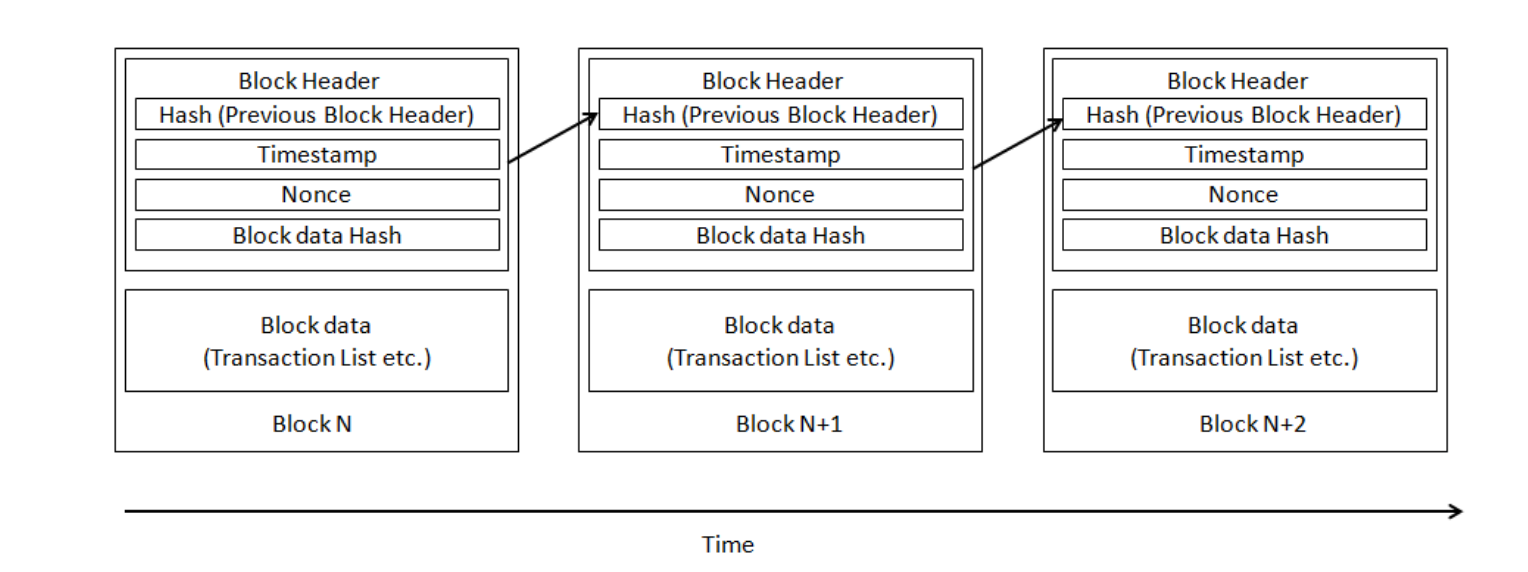
\includegraphics[width=1.95\textwidth]{images/chap01_BlockChain.png}
		\end{minipage}
		\caption[Block contents]{Block contents}
		
	\end{figure}
	
\end{center}
\begin{itemize}
    \item \textbf{Block}
    The data stored in the block contains different functions which include transaction hashes and some other additional information for blockchain technology. \textit{Gavin Wood} described some relevant information as bellow and we used this information in our project: \\
    \begin{itemize}
        \item \textit{parentHash}: The hash of the parent block’s header.
        \item \textit{sateRoot}: The hash of the root node of the state, after transactions are executed.
        \item \textit{transactionRoot}: The hash of the root node of data populated with a transaction in the transactions list inside the block.
        \item \textit{receiptRoot}: The hash of the root node of the data populated with the receipts of transactions in the block.
        \item \textit{logsBloom} composed of log information.
        \item \textit{difficulty} represents the difficulty level of the block.
        \item \textit{number} is the number of ancestor blocks.
        \item \textit{gasLimit} represents the current limit of gas in the block.
        \item \textit{gasUsed} is the amount of gas used for the transaction in the block.
        \item \textit{timestamp}
        \item \textit{extraData} is a byte array containing relevant information in the block.
        \item \textit{nonce} is several computations that have been done in the block.
    \end{itemize}
    \item \textbf{mining}
    It is a process of computation on the blockchain to verify and add a block. Miner adds a new block and others check the validity of the new block. Any participant can take part in the mining pool, But the chance of finding valid block depends on the power of the computer to perform calculations. Sometimes a miner will find an uncle block; an uncle block is a block that is initially valid but is surpassed by another faster block. Uncle block is rewarded with $\frac{7}{8}$ of full block value and hash will be added to a valid block. A max of two uncle blocks can add to a valid block and the miner of the valid block also receive $\frac{1}{32}$ extra Ether for each uncle block\cite{Egbertsen}.
    \item \textbf{mining pool}
     Mining can be done alone or in the mining pool. A mining pool is a better way to solve a block and get rewards as compared to mining alone. Miners in the pool mine together and rewards will be split to all members in the pool\cite{Egbertsen}.
\end{itemize}
\subsection{Ether}
 Is the form of payment and fuel for Ethereum. The base for mining (find the solution and add block) successfully mining block is five Ether. If the miner finds a solution but not fast, it becomes less ether like 4.375 Ether, and will be uncle block. Each block can contain just two uncle blocks and receive $\frac{1}{32}$ per uncle block. If another miner also finds a solution. this block can not be added to the blockchain and the miner just receives 2-3 Ether\cite{Egbertsen}. 
\subsection{Account}
There are two types of accounts in Ethereum:\\
- \textit{Normal account} is controlled by the private key. The owner of this account can send Ether or a message.\\
- \textit{Contract} account is controlled by code. It can only fire a transaction in response to other transactions.\cite{Egbertsen}. An account encompasses four fields:\\
 \begin{itemize}
     \item \textit{nonce} is the number of transactions sent from this address \cite{Gavin}.
     \item \textit{balance} is the number of Wei owned by this address\cite{Gavin}.
     \item \textit{storageRoot} is the hash of the root node of the Merkle Patrica tree which encodes the content of an account. It should be also not that the Merkle tree is used for data representation in block header\cite{Gavin}.
     \item \textit{codeHash}
     The hash associated with this account would be executed when this account address receives a message call and would not be changeable anymore. All information about this account is stored in the database under the corresponding hash code for later retrieval. \\
    
\end{itemize}
\textbf{Hash function}
The process of SHA-3 standardization by NIST was completed in Auguts 2015.
This standard specify SHA3 (Secure hash algorithm-3) family of function on binary data. Each hash function is based on \textit{Kacak} algorithm that is known as NIST as winner of SHA-3 cryptographic hash algorithm competition. The SHA3 family includes four functions with different lengths of 224, 256, 384, and 512 bits. 
In hash function, input called as \textit{message} and output called as  \textit{has value} which the length of message can vary but, the length of hash value is always fixed \cite{Fips}.\\

\begin{center}
	\begin{figure}[htb!]
		
		\begin{minipage}{0.2\linewidth}
			\centering
			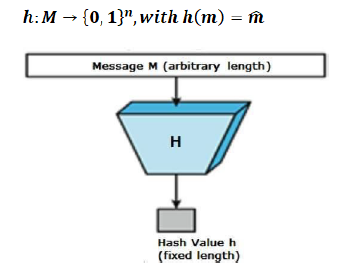
\includegraphics[width=4.5\textwidth]{images/chap01_hash_function.png}
		\end{minipage}
		\caption[Image of hash function]{Image of hash function}
		
	\end{figure}
	
\end{center}
\textbf{Gas} Transaction in the Ethereum platform needs fuel to execute called gas which is used internally and paid in advance to execute a transaction. If the transaction gets run off gas, means the transaction is executed. If the transaction rolled back but consumed gas will not be returned.\\
To enable easier calculations, Ether also has some sub-denominations\cite{Egbertsen}:\\
\begin{itemize}
	\item Wei - $10^0$
	\item Szabo - $10^12$
	\item Finney - $10^15$
	\item Ether - $10^18$
\end{itemize}
\begin{itemize}
    \item \textbf{Transaction}
     \textit{Gavin Wood} described a transaction as a cryptography-signed instruction that is executed by an external actor. An external actor can be a human or another contract. Transaction describes these fields:
     \begin{itemize}
         \item \textit{nonce} is the number of transactions sent by the sender.
         \item \textit{gasPrice} is the number of Wei to be paid per unit of gas.
         \item \textit{gasLimit} is the amount of gas that can be used for transactions.
         \item \textit{to} is the address to which that contract sends a transaction.
         \item \textit{value} is the number of Wei that is transferred in the transaction.
     \end{itemize}
        \item \textbf{Message}
        As already said blockchain fires transactions when receiving a transaction. When an account sends a transaction means sending a message. The message contains all attributes the same as a transaction, but $gasPrice$. the only difference between message and transaction is that message is fired by contract\cite{Egbertsen}.
\end{itemize}
\subsection{Contracts} is an account in the Ethereum blockchain having its code and controlled by code. The code inside the contract is triggered whenever it receives a message, allowing it to read and write contract storage or send a message. \\
A contract in Ethereum is an autonomous agent that performs some operations which are programmed to fulfill the user's goals, meaning that the contract is an alive autonomous agent which is executed when it receives a message or transaction, having control over its balance and the key /value store to constant variables.
the key and values stored in the contract are long-lasting and get used whenever the contract starts running \cite{Egbertsen}.

\subsection{smart contract}
 The term smart contract was coined in 1994 by Nick Szabo who released that DLT can be used for smart contracts. 
According to Nick Szabo \textit{A smart contract is a computerized transaction protocol that executes the terms of  a contract}\footnote{https://www.fon.hum.uva.nl/rob/Courses/InformationInSpeech/CDROM/Literature/LOTwinterschool2006/szabo.best.vwh.net/smart.contracts.html}. He visualized an away to write agreement which enforces the conditions between parties involved in transaction automatically and more efficiently.
Smart contracts run by each node as part of the block creation process. Block creation means when transactions take place in the block.
An important part of a smart contract is that each contract has its address. Since the contract code is con carried to the transaction, a node can create the spacial transaction, assigning an address to the contract, then this transaction is capable to run contract code at the time of creation.\\
After that, the contract will be part of the block and the address will never change. Whenever the node wants to call a method inside the contract, should send a message to the address of the contract having the method and input data.
the contract will run as the part of creation of a new block, then return value or store data in the blockchain. \cite{Payrott}.

\textbf{Solidity} is high-level truing complete language with Java script similar syntax. The contract is similar to classes in an object-oriented language which contains the fields as persistent storage of contracts and methods to be invoked by internal and external transactions. For interacting with another contract, you either need to create a new instance of this contract or make a transaction to a known contract address.\\
In principle, Solidity provides some basics to access blocks and transactions details like: \textit{msg:sender} for accessing the address of an account or \textit{msg:value} to access the amount of \textit{wei} transferred by the transaction. Solidity uses some functions to transfer money to another contract such as \textit{call} and \textit{send}. This function gets used to transfer value and translate as an internal call to a transaction which causes to call contract also execute code or may fail to execute due to insufficient gas \cite{Ilya}.

